\section{\RU{Проверка результата scanf()}\EN{scanf() result checking}}

\RU {Как я уже упоминал, использовать \scanf в наше время слегка старомодно. 
Но если уж жизнь заставила этим заниматься, нужно хотя бы проверять, сработал ли \scanf 
правильно или пользователь ввел вместо числа что-то другое, что \scanf не смог трактовать как число.}
\EN{As I noted before, it is slightly old-fashioned to use \scanf today. 
But if we have to, we need to at least check if \scanf finishes correctly without an error.}

\lstinputlisting{patterns/04_scanf/3_checking_retval/ex3.c}

\RU{По стандарту,}\EN{By standard, the} 
\scanf\footnote{scanf, wscanf: \href{http://go.yurichev.com/17255}{MSDN}} 
\RU{возвращает количество успешно полученных значений.}
\EN{function returns the number of fields it has successfully read.}

\RU{В нашем случае, если всё успешно и пользователь ввел таки некое число, \scanf вернет 1. 
А если нет, то 0 (или \ac{EOF}).} 
\EN{In our case, if everything goes fine and the user enters a number 
\scanf returns 1, or in case of error (or \ac{EOF}) --- 0.}

\RU{Я добавил код, проверяющий результат \scanf и в случае ошибки он сообщает пользователю что-то другое.}
\EN{I have added some C code to check the \scanf return value and print error message in case of an error.}

\RU{Это работает предсказуемо}\EN{This works as expected}:

\begin{lstlisting}
C:\...>ex3.exe
Enter X:
123
You entered 123...

C:\...>ex3.exe
Enter X:
ouch
What you entered? Huh?
\end{lstlisting}

% subsections
\subsection{MSVC: x86}

\RU{Вот, что выходит на ассемблере}\EN{What we got in assembly language} (MSVC 2010):

\lstinputlisting{patterns/04_scanf/3_checking_retval/ex3_MSVC_x86.asm}

\index{x86!\Registers!EAX}
\RU{Для того чтобы вызывающая функция имела доступ к результату вызываемой функции, 
вызываемая функция (в нашем случае \scanf) оставляет это значение в регистре \EAX.}
\EN{\Gls{caller} function (\main) must have access to the result of \gls{callee} function (\scanf), 
so \gls{callee} leaves this value in the \EAX register.}

\index{x86!\Instructions!CMP}
\RU{Мы проверяем его инструкцией \TT{CMP EAX, 1} (\IT{CoMPare}), то есть, 
сравниваем значение в \EAX с 1.}
\EN{After, we check it with the help of instruction \TT{CMP EAX, 1} (\IT{CoMPare}),
in other words, we compare value in the \EAX register with $1$.} 

\index{x86!\Instructions!JNE}
\RU{Следующий за инструкцией \CMP: условный переход \JNE. 
Это означает \IT{Jump if Not Equal}, то есть, условный переход \IT{если не равно}.}
\EN{\JNE conditional jump follows \CMP instruction. \JNE means \IT{Jump if Not Equal}.}

\RU{Итак, если \EAX не равен 1, то \JNE заставит перейти процессор 
по адресу указанном в операнде \JNE, у нас это \TT{\$LN2@main}.}
\EN{So, if value in the \EAX register not equals to $1$, then the processor will pass execution to the 
address mentioned in operand of \JNE, in our case it is \TT{\$LN2@main}.}
\RU{Передав управление по этому адресу, \ac{CPU} как раз начнет исполнять вызов \printf с 
аргументом \TT{``What you entered? Huh?''}.}
\EN{Passing control to this address, \ac{CPU} will execute function \printf 
with argument \TT{``What you entered? Huh?''}.}
\RU{Но если все нормально, перехода не случится, и исполнится другой \printf с двумя аргументами: 
\TT{'You entered \%d...'} и значением переменной \TT{x}.}
\EN{But if everything is fine, conditional jump will not be taken, and another \printf call 
will be executed, with two arguments: \TT{'You entered \%d...'} and value of variable \TT{x}. }

\index{x86!\Instructions!XOR}
\index{\CLanguageElements!return}
\RU{А для того чтобы после этого вызова не исполнился сразу второй вызов \printf, 
после него имеется инструкция \JMP, безусловный переход, он отправит процессор на место аккурат 
после второго \printf и перед инструкцией \TT{XOR EAX, EAX}, которая собственно \TT{return 0}.}
\EN{Since second subsequent \printf not needed to be executed, there is \JMP after (unconditional jump),
it will pass control to the point after second \printf and before \TT{XOR EAX, EAX} instruction, 
which implement \TT{return 0}.}

\index{x86!\Registers!\Flags}
\RU{Итак, можно сказать, что в подавляющих случаях сравнение какой-либо переменной с чем-то другим 
происходит при помощи пары инструкций \CMP и \Jcc, где \IT{cc} это \IT{condition code}.}
\EN{So, it can be said that comparing a value with another is \IT{usually} implemented
by \CMP/\Jcc instructions pair, where \IT{cc} is \IT{condition code}.}
\RU{\CMP сравнивает два значения и выставляет 
флаги процессора\footnote{См. также о флагах x86-процессора: \url{http://en.wikipedia.org/wiki/FLAGS_register_(computing)}.}.}
\EN{\CMP comparing two values and set 
processor flags\footnote{About x86 flags, see also: \url{http://en.wikipedia.org/wiki/FLAGS_register_(computing)}.}.}
\RU{\Jcc проверяет нужные ему флаги и выполняет переход по указанному адресу (или не выполняет).}
\EN{\Jcc check flags needed to be checked and pass control to mentioned address (or not pass).}

\index{x86!\Instructions!CMP}
\index{x86!\Instructions!SUB}
\label{CMPandSUB}
\RU{Но на самом деле, как это не парадоксально поначалу звучит, \CMP это почти то же самое что и 
инструкция \SUB, которая отнимает числа одно от другого.}
\EN{But in fact, this could be perceived paradoxical, but \CMP instruction is in fact \SUB (subtract).}
\RU{Все арифметические инструкции также выставляют флаги в соответствии с результатом, не только \CMP.}
\EN{All arithmetic instructions set processor flags too, not just \CMP.}
\RU{Если мы сравним 1 и 1, от единицы отнимется единица, получится $0$, и выставится флаг 
\ZF (\IT{zero flag}), означающий что последний полученный результат был $0$.}
\EN{If we compare 1 and 1, $1-1$ will be $0$ in result, \ZF flag will be set (meaning the last result was $0$).}
\RU{Ни при каких других значениях \EAX, флаг \ZF выставлен не будет, кроме тех, когда операнды равны друг другу.}
\EN{There is no any other circumstances when it is possible except when operands are equal.}
\index{x86!\Instructions!JNE}
\index{x86!\Registers!ZF}
\RU{Инструкция \JNE проверяет только флаг \ZF, и совершает переход только если флаг не поднят. 
Фактически, \JNE это синоним инструкции \JNZ (\IT{Jump if Not Zero}).}
\EN{\JNE checks only \ZF flag and jumping only if it is not set. 
\JNE is in fact a synonym of \JNZ (\IT{Jump if Not Zero}) instruction.}
\RU{Ассемблер транслирует обе инструкции в один и тот же опкод.}
\EN{Assembler translating both \JNE and \JNZ instructions into same opcode.}
\RU{Таким образом, можно \CMP заменить на \SUB и все будет работать также, но разница в том, что \SUB 
все-таки испортит значение в первом операнде. \CMP это \IT{SUB без сохранения результата}.}
\EN{So, \CMP instruction can be replaced to \SUB instruction and almost everything will be fine,
but the difference is in 
the \SUB alter the value of the first operand.
\CMP is \IT{SUB without saving result}.}

\ifx\LITE\undefined
\subsection{MSVC: x86: IDA}

\index{IDA}
\RU{Наверное, уже пора делать первые попытки анализа кода в \IDA}
\EN{It's time to run \IDA and try to do something in it}.
\RU{Кстати, для начинающих, полезно компилировать в MSVC с ключом \TT{/MD}, что означает что все эти стандартные
ф-ции не будут скомпонованы с исполняемым файлу, а будут импортироваться из файла \TT{MSVCR*.DLL}}
\EN{By the way, it is good idea to use \TT{/MD} option in MSVC for beginners: this mean that all these
standard functions will not be linked with executable file, but will be imported from the \TT{MSVCR*.DLL}
file instead}.
\RU{Так будет легче увидеть, где какая стандартная ф-ция используется}\EN{Thus it will be easier to see
which standard function used and where}.

\RU{Анализируя код в \IDA, очень полезно делать пометки для себя (и других)}
\EN{While analysing code in \IDA, it is very advisable to do notes for oneself (and others)}.
\RU{Например, разбирая этот пример, мы сразу видим что \TT{JNZ} срабатывает в случае ошибки}
\EN{For example, analysing this example, we see that \TT{JNZ} will be triggered in case of error}.
\RU{Можно навести курсор на эту метку, нажать ``n'' и переименовать метку в ``error''}
\EN{So it's possible to move cursor to the label, press ``n'' and rename it to ``error''}.
\RU{Еще одну метку}\EN{Another label}\EMDASH{}\RU{в}\EN{into} ``exit''.
\RU{Вот как у меня получилось в итоге}\EN{What I've got}:

\lstinputlisting{patterns/04_scanf/3_checking_retval/ex3.lst}

\RU{Так понимать код становится чуть легче}\EN{Now it's slightly easier to understand the code}.
\RU{Впрочем, меру нужно знать во всем и комментировать каждую инструкцию не стоит}
\EN{However, it's not good idea to comment every instruction excessively}.

% FIXME draw button?
\RU{В \IDA также можно скрывать части ф-ций: нужно отметить часть, нажать ``--'' на цифровой клавиатуре и ввести
текст}\EN{A part of function can also be hidden in \IDA: a block should be marked, then ``--'' on numerical pad
is pressed and text to be entered}.

\RU{Я скрыл две части и придумал им названия}\EN{I've hide two parts and gave names to them}:

\lstinputlisting{patterns/04_scanf/3_checking_retval/ex3_2.lst}

% FIXME draw button?
\RU{Раскрывать скрытые части ф-ций можно при помощи ``+'' на цифровой клавиатуре}
\EN{To unhide these parts, ``+'' on numerical pad can be used}.

\clearpage
\RU{Нажав ``пробел'', мы увидим как \IDA может представить ф-цию в виде графа}\EN{By pressing ``space'',
we can see how \IDA can represent a function as a graph}:

\begin{figure}[H]
\centering
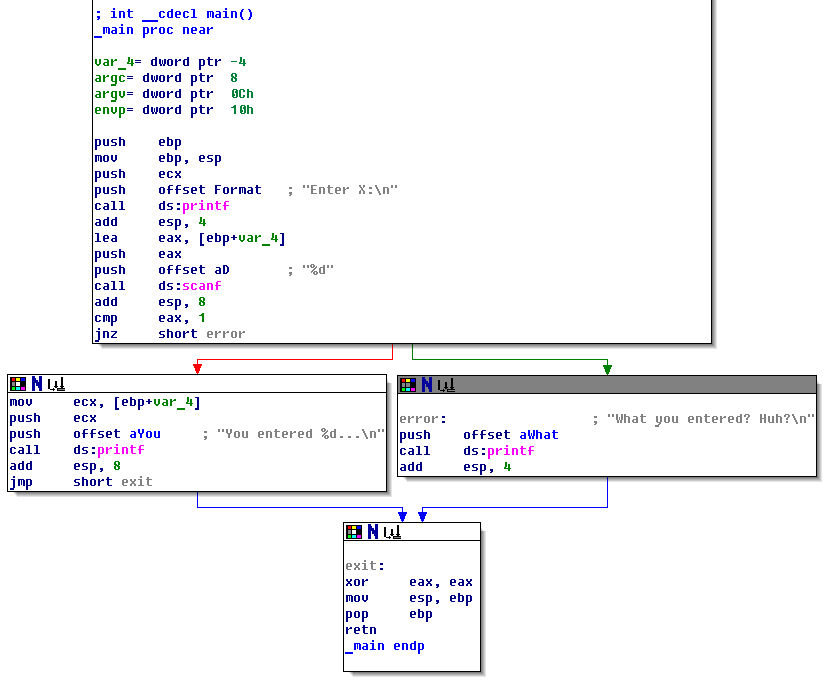
\includegraphics[scale=\FigScale]{patterns/04_scanf/3_checking_retval/IDA.png}
\caption{\RU{Отображение в IDA в виде графа}\EN{Graph mode in IDA}}
\label{fig:ex3_IDA_1}
\end{figure}

\RU{После каждого условного перехода видны две стрелки: зеленая и красная}\EN{There are two arrows
after each conditional jump: green and red}.
\RU{Зеленая ведет к тому блоку, который исполнится если переход сработал, а красная --- если не сработал}
\EN{Green arrow pointing to the block which will be executed if jump is triggered, and red if otherwise}.

\clearpage
\RU{В этом режиме также можно сворачивать узлы и давать им названия}
\EN{It is possible to fold nodes is this mode and give them names as well} (``group nodes'').
\RU{Я сделал это для трех блоков}\EN{I did it for 3 blocks}:

\begin{figure}[H]
\centering
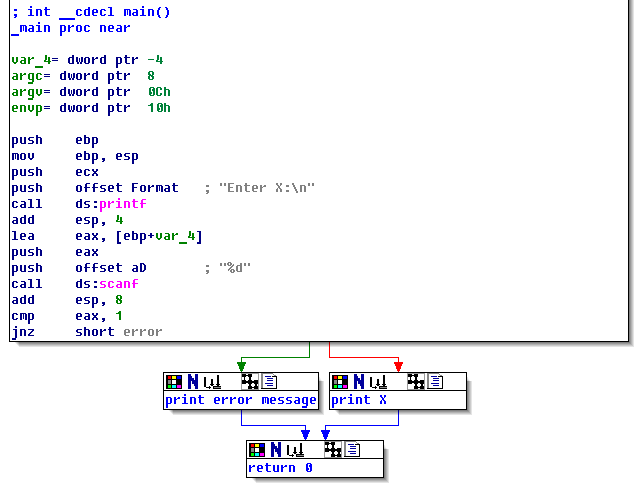
\includegraphics[scale=\FigScale]{patterns/04_scanf/3_checking_retval/IDA2.png}
\caption{\RU{Отображение в IDA в виде графа с тремя свернутыми блоками}\EN{Graph mode in IDA with 3 nodes folded}}
\label{fig:ex3_IDA_2}
\end{figure}

\RU{Всё это очень полезно делать}\EN{It's very useful}.
\RU{Вообще, очень важная часть работы реверсера состоит в том, чтобы уменьшать количество имеющейся информации}
\EN{It can be said, a very important part of reverse engineer's job is to reduce information he/she have}.
\fi

\ifdefined\IncludeOlly
\clearpage
\subsection{MSVC: x86 + \olly}

\RU{Попробуем в \olly немного хакнуть программу, и сделать вид что \scanf срабатывает всегда без ошибок}
\EN{Let's try to hack our program in \olly, forcing it to think \scanf working always without error}.

\RU{Когда в \scanf передается адрес локальной перемейнной, изначальное, в данном случае, 
у нас в этой переменной
находится некий мусор, а это}\EN{When address of local variable is passed into \scanf,
initially this variable contain some random garbage, that is} \TT{0x4CD478}\EN{ in case}:

\begin{figure}[H]
\centering
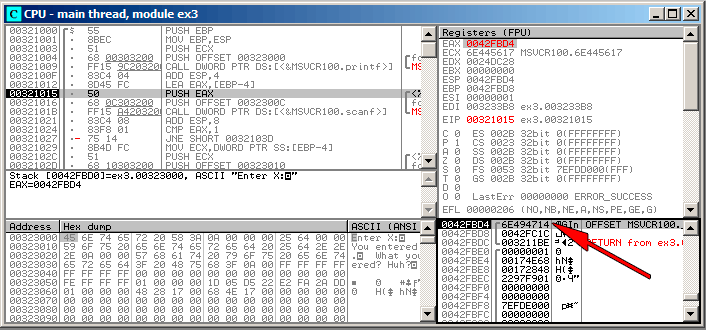
\includegraphics[scale=\FigScale]{patterns/04_scanf/3_checking_retval/olly_1.png}
\caption{\olly: \RU{передача адреса переменной в}\EN{passing variable address into} \scanf}
\label{fig:scanf_ex3_olly_1}
\end{figure}

\clearpage
\RU{Когда}\EN{When} \scanf \RU{запускается, я ввожу в консоли что-то непохожее на число, например}
\EN{is executing, I entered something definitely not a number in the console, like} ``asdasd''.
\scanf \RU{заканчивается с 0 в}\EN{finishing with 0 in} \EAX, \RU{что означает, что произошла ошибка}
\EN{which mean, an error occurred}:

\begin{figure}[H]
\centering
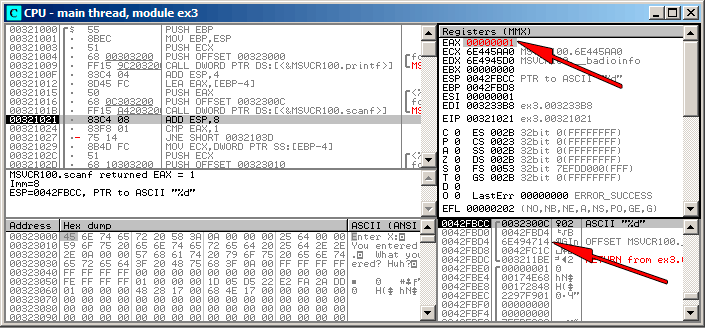
\includegraphics[scale=\FigScale]{patterns/04_scanf/3_checking_retval/olly_2.png}
\caption{\olly: \scanf \RU{закончился с ошибкой}\EN{returning error}}
\label{fig:scanf_ex3_olly_2}
\end{figure}

\RU{Вместе с этим, мы можем посмотреть на локальную переменную в стеке, она не изменилась}
\EN{We can also see to the local variable in the stack and notice that it's not changed}.
\RU{Действительно, ведь что туда записала бы ф-ция \scanf}\EN{Indeed, what \scanf would write there}?
\RU{Она просто ничего не делала кроме возвращения нуля}\EN{It just did nothing except returning zero}.

\clearpage
\RU{Теперь попробуем немного ``хакнуть'' нашу программу}\EN{Now let's try to ``hack'' our program}.
\RU{Кликнем правой кнопкой на}\EN{Let's right-click on} \EAX, \RU{там, в числе опций, будет также}
\EN{there will also be} ``Set to 1''\EN{ among other options}.
\RU{Это то что нам нужно}\EN{This is what we need}.

\RU{В \EAX теперь 1, последующая проверка пройдет как надо, и \printf выведет значение переменной
из стека}\EN{1 now in \EAX, so the following check will executed as we need, and \printf will print
value of variable in the stack}.

\RU{Запускаем}\EN{Let's run} (F9) \RU{и видим в консоли следующее}\EN{and we will see this in 
console window}:

\begin{figure}[H]
\centering
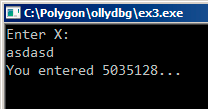
\includegraphics[scale=\FigScale]{patterns/04_scanf/3_checking_retval/olly_3.png}
\caption{\RU{консоль}\EN{console window}}
\end{figure}

\RU{Действительно}\EN{Indeed}, $5035128$ \RU{это десятичное представление числа в стеке}
\EN{is a decimal representation of the number in stack} (\TT{0x4CD478})!

\clearpage
\subsection{MSVC: x86 + Hiew}
\index{Hiew}

\RU{Это еще и может быть простым примером патчинга исполняемого файла}\EN{This can be 
also a simple example of executable file patching}.
\RU{Мы можем попробовать пропатчить его таким образом, что программа всегда будет выводить числа,
вне зависимости от того, что мы вводим}\EN{We may try to patch executable, so the program will always 
print numbers, no matter what we entered}.

\RU{Учитывая, что исполняемый файл скомпилирован с учетом импортирования ф-ций из}\EN{Assuming the 
executable compiled against external} \TT{MSVCR*.DLL} (\RU{т.е., с опцией}\EN{i.e., with} 
\TT{/MD}\EN{ option})\footnote{\RU{то, что еще называют}\EN{that's what also called} ``dynamic linking''}, 
\RU{мы можем отыскать ф-цию}\EN{we may find} \main \RU{в самом начале секции}\EN{function at the 
very beginning of} \TT{.text}\EN{ section}.
\RU{Откроем исполняемый файл в Hiew, найдем самое начало секции}\EN{Let's open executable in Hiew, 
find the very beginning of} \TT{.text}\EN{ section} (Enter, F8, F6, Enter, Enter).

\RU{Мы увидим следующее}\EN{We will see this}:

\begin{figure}[H]
\centering
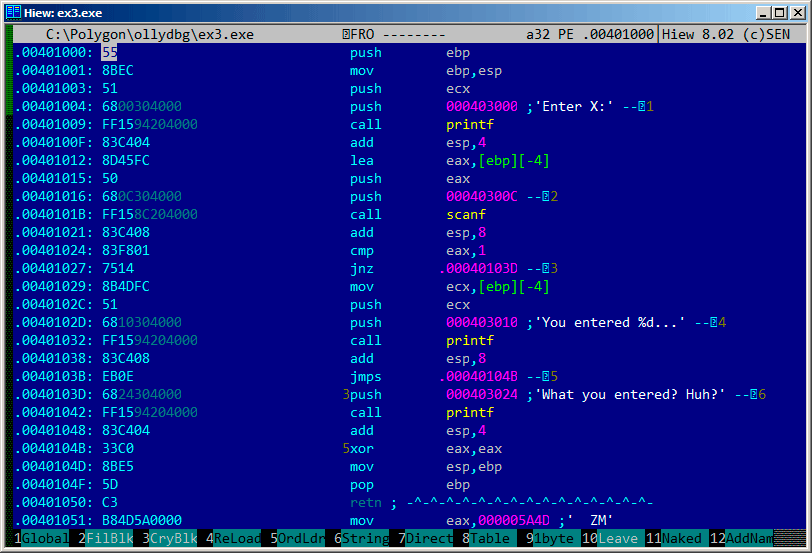
\includegraphics[scale=\FigScale]{patterns/04_scanf/3_checking_retval/hiew_1.png}
\caption{Hiew: \RU{ф-ция }\main\EN{ function}}
\label{fig:scanf_ex3_hiew_1}
\end{figure}

Hiew \RU{находит}\EN{finds} \ac{ASCIIZ}\RU{-строки и показывает их, также как и имена импортируемых 
ф-ций}\EN{ strings and displays them, as well as imported function names}.

\clearpage
\RU{Переведите курсор на адрес}\EN{Move cursor to the address} \TT{.00401027} 
(\RU{с инструкцией}\EN{with the} \TT{JNZ}\RU{, которую мы хотим заблокировать}\EN{ instruction we 
should bypass}), \RU{нажмите}\EN{press} F3,
\RU{затем наберите}\EN{and then type} ``9090'' (\RU{что означает}\EN{meaning two} \ac{NOP}-\RU{а}\EN{s}): 

\begin{figure}[H]
\centering
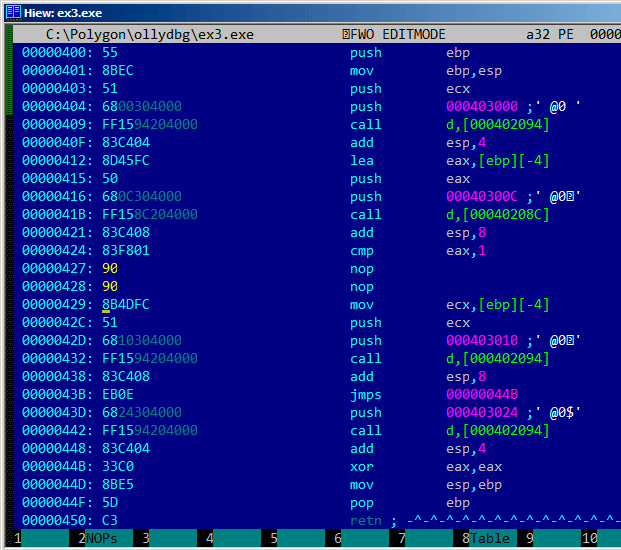
\includegraphics[scale=\FigScale]{patterns/04_scanf/3_checking_retval/hiew_2.png}
\caption{Hiew: \RU{замена}\EN{replacing} \TT{JNZ} \RU{на два}\EN{by two} \ac{NOP}-\RU{а}\EN{s}}
\label{fig:scanf_ex3_hiew_2}
\end{figure}

\RU{Затем}\EN{Then} F9 (update). \RU{Теперь исполняемый файл записан на диск. Он будет вести себя
так, как нам надо.}\EN{Now the executable saved to disk. It will behave as we wanted.}

\RU{Два}\EN{Two} \ac{NOP}-\RU{а}\EN{s} \RU{возможно, не так эстетично, как могло бы быть}\EN{are probably 
not quite \ae{}sthetically as it could be}.
\RU{Другой способ пропатчить инструкцию, это записать 0 во второй байт опкода (смещение перехода),
так что}\EN{Other way to patch this instruction is to write just 0 to the second opcode byte (\gls{jump offset}), 
so that} \TT{JNZ} \RU{всегда будет переходить на следующую инструкцию}\EN{will always jump to 
the next instruction}.

\RU{Можно пропатчить и наоборот: первый байт заменить на \TT{EB}, второй байт (смещение перехода) 
не трогать}
\EN{We can do the opposite: replace first byte to \TT{EB} while not touching the second byte (\gls{jump offset})}.
\RU{Получится всегда срабатывающий безусловный переход}\EN{We'll got here always triggered unconditional
jump}.
\RU{Теперь сообщение об ошибке будет выдаваться всегда, даже если мы ввели число}
\EN{The error message will be printed always, no matter what number was entered}.

\fi

\subsection{MSVC: x64}

\myindex{x86-64}

\ifdefined\RUSSIAN
Так как здесь мы работаем с переменными типа \Tint, а они в x86-64 остались 32-битными, то мы здесь видим, как продолжают использоваться регистры с префиксом \TT{E-}.
Но для работы с указателями, конечно, используются 64-битные части регистров с префиксом \TT{R-}.
\fi

\ifdefined\ENGLISH
Since we work here with \Tint{}-typed variables, which are still 32-bit in x86-64, we see how the 32-bit part of the registers (prefixed with \TT{E-}) are used here as well.
While working with pointers, however, 64-bit register parts are used, prefixed with \TT{R-}.
\fi

\ifdefined\BRAZILIAN
Como trabalhamos aqui com variáveis do tipo \Tint, que ainda são 32-bits no x86-64, nós vemos como a parte de 32-bits dos registradores (com o prefixo \TT{E-}) sao usadas aqui da mesma maneira.
No entanto, quando trabalhamos com ponteiros, as partes dos registradores de 64-bits são usadas, prefixadas com \TT{R-}.
\fi

\lstinputlisting[caption=MSVC 2012 x64]{patterns/04_scanf/3_checking_retval/ex3_MSVC_x64.asm.\LANG}


\ifdefined\IncludeARM
\subsection{ARM}

\subsubsection{ARM: \OptimizingKeilVI (\ThumbMode)}

\lstinputlisting[caption=\OptimizingKeilVI (\ThumbMode)]{patterns/04_scanf/3_checking_retval/ex3_ARM_Keil_thumb_O3.asm}

\index{ARM!\Instructions!CMP}
\index{ARM!\Instructions!BEQ}
\RU{Новые инструкции здесь для нас: \CMP и \ac{BEQ}.}
\EN{New instructions here are \CMP and \ac{BEQ}.}

\CMP \RU{аналогична той что в x86, она отнимает один аргумент от второго и сохраняет флаги.}
\EN{is akin to the x86 instruction bearing the same name, it subtracts one argument from another and saves flags.}
% TODO: в мануале ARM $op1 + NOT(op2) + 1$ вместо вычитания

\index{ARM!\Registers!Z}
\index{x86!\Instructions!JZ}
\ac{BEQ} \RU{совершает переход по другому адресу, 
если операнды при сравнении были равны, 
либо если результат последнего вычисления был $0$, либо если флаг Z равен $1$.}
\EN{is jumping to another address if operands while comparing were equal to each other, or,
if result of last computation was $0$, or if Z flag is $1$.}
\RU{То же что и \JZ в}\EN{Same thing as \JZ in} x86.

\RU{Всё остальное просто: исполнение разветвляется на две ветки, затем они сходятся там, 
где в \Reg{0} записывается $0$ как возвращаемое из функции значение и происходит выход из функции.}
\EN{Everything else is simple: execution flow is forking into two branches, then the branches are 
converging at the point
where $0$ is written into the \Reg{0}, as a value returned from the function, and then function finishing.}

\subsubsection{ARM64}

\lstinputlisting[caption=\NonOptimizing GCC 4.9.1 ARM64,numbers=left]{patterns/04_scanf/3_checking_retval/ARM64_GCC491_O0.s}

\index{ARM!\Instructions!CMP}
\index{ARM!\Instructions!Bcc}
\EN{Code flow is divided here using CMP/BNE (Branch if Not Equal) instructions pair.}
\RU{Исполнение здесь разветвляется используя пару инструкций CMP/BNE (Branch if Not Equal: переход если не равно).}

\fi
\ifdefined\IncludeMIPS
\subsection{MIPS}

\lstinputlisting[caption=\Optimizing GCC 4.4.5 (IDA)]{patterns/04_scanf/3_checking_retval/MIPS_O3_IDA.lst}

\index{MIPS!\Instructions!BEQ}
\RU{\scanf возвращает результат своей работы в регистре \$V0 и он проверяется по адресу 0x004006E4
сравнивая значения в \$V0 и \$V1 (1 записан в \$V1 раннее, на 0x004006DC).}
\EN{\scanf returns the result of its work in register \$V0. It is checked at address 0x004006E4
by comparing the values in \$V0 with \$V1 (1 was stored in \$V1 earlier, at 0x004006DC).}
BEQ \EN{stands for}\RU{означает} ``Branch Equal''\RU{ (переход если равно)}.
\RU{Если значения равны (т.е., в случае успеха), произойдет переход по адресу 0x0040070C.}
\EN{If the two values are equal (i.e., success), the execution jumps to address 0x0040070C.}

\fi

\ifdefined\IncludeExercises
\subsection{\Exercise}

\index{x86!\Instructions!Jcc}
\index{ARM!\Instructions!Bcc}
\EN{As we can see, the JNE/JNZ instruction can be easily replaced by the JE/JZ and vice versa 
(or BNE by BEQ and vice versa).}
\RU{Как мы можем увидеть, инструкцию JNE/JNZ можно вполне заменить на JE/JZ или наоборот 
(или BNE на BEQ и наоборот).}
\EN{But then the basic blocks must also be swapped.}\RU{Но при этом ещё нужно переставить базовые блоки местами.}
\EN{Try to do this in some of the examples.}\RU{Попробуйте сделать это в каком-нибудь примере.}
\fi
